\input{header}

\AtBeginSubsection[]
{
	\begin{frame}<beamer>
		\frametitle{Outline}
		\tableofcontents[current,currentsubsection]
	\end{frame}
}

\begin{document}



\begin{frame}[allowframebreaks] 
\frametitle{Pushdown automata}
\begin{itemize}
\item Context-free languages are more general than regular
  languages
\item For regular languages, by definition, there are automata to
  recognize them
\item What are machines to recognize CFL?
\item Pushdown automata (PDA)

\item [] It's more powerful by having a \alert{stack}
\item DFA (or NFA):
\begin{center}
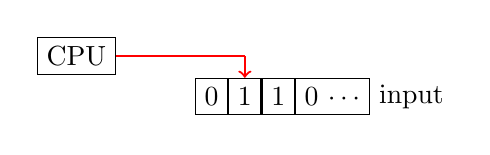
\begin{tikzpicture}[ampersand replacement=\&]
\matrix 
{
  \node[draw](0) {CPU}; \& [1cm] \& \node(1){}; \&\&\& \\
  \& \node[draw]{0}; \& \node[draw](a){1}; \& \node[draw]{1}; \& \node[draw]{0 $\cdots$};  \& \node{input};\\
};
\draw [-,red,thick] (0) -- (1.center) ;
\draw [->,red,thick] (1.center) -- (a) ;
\end{tikzpicture}
\end{center}
\item Pushdown automata:
\begin{center}
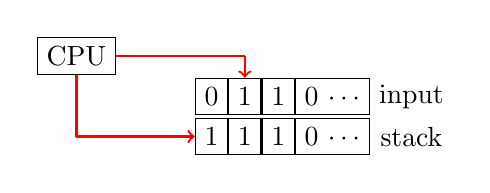
\begin{tikzpicture}[ampersand replacement=\&]
\matrix 
{
  \node[draw](0) {CPU}; \& [1cm]  \& \node(1){} ; \&\&\& \\
  \& \node[draw]{0}; \& \node[draw](a){1}; \& \node[draw]{1}; \& \node[draw]{0 $\cdots$};  \& \node{input};\\
\node(c){}; \& \node[draw](b){1}; \& \node[draw]{1}; \& \node[draw]{1}; \& \node[draw]{0 $\cdots$}; \&  \node{stack}; \\
};

\draw [-,red,thick] (0) -- (1.center) ;
\draw [->,red,thick] (1.center) -- (a) ;
\draw [-,red,thick] (0) -- (c.center) ;
\draw [->,red,thick] (c.center) -- (b) ;
\end{tikzpicture}
\end{center}

\item What is a stack?

\item [] We know they are like plates in a cafeteria

\item [] An important property: \alert{last in first out}
\item Let's see how stack can help to recognize
  \begin{equation*}
\{0^n 1^n\mid n \geq 0\}
\end{equation*}
\item If 0 is read, 0 is pushed to stack
\item If 1 is read, 0 is popped up
\item By checking (0, 1) pairs, we know if the input is
  $0^n 1^n$
\end{itemize}
\end{frame}

\begin{frame}[allowframebreaks] \frametitle{Example 2.14}
  \begin{itemize}
  \item Consider the following language
    \begin{equation*}
    \{0^n 1^n\mid n \geq 0\}
  \end{equation*}

\begin{center}
\begin{tikzpicture}
\node[state,initial,accepting] (q_1) {$q_1$};
\node[state] (q_2) [right of=q_1] {$q_2$};
\node[state] (q_3) [below of=q_2] {$q_{3}$};
\node[state,accepting] (q_4) [left of=q_3] {$q_{4}$};      
  \path 
  (q_1) edge[above]  node {$\epsilon, \epsilon \rightarrow \$ $} (q_2)
  (q_2) edge[loop right]  node {$0,\epsilon \rightarrow 0$} (q_2)
  (q_2) edge[right]  node {$1, 0 \rightarrow \epsilon$} (q_3)
  (q_3) edge[loop right]  node {$1, 0 \rightarrow \epsilon$} (q_3)  
  (q_3) edge[below] node {$\epsilon, \$ \rightarrow \epsilon$} (q_4);
  \end{tikzpicture}
\end{center}
\item \$: a special symbol to indicate the initial state of stack

  
\item How it works:
  \item [] $q_2 \rightarrow q_2$, put 0 into stack

  \item [] $q_2 \rightarrow q_3$ and $q_3 \rightarrow q_3$, read 1 and  pop 0 up
  \item The input
  \begin{equation*}
    0011
  \end{equation*}
is the same as
  \begin{equation*}
    \epsilon 0011 \epsilon
  \end{equation*}
\item Steps:
  \begin{equation*}
    \begin{split}
& q_1, \emptyset, \epsilon\\
& q_2, \{\$\}, 0 \\
& q_2, \{0,\$\}, 0\\
& q_2, \{0,0,\$\}, 1\\
& q_3, \{0,\$\}, 1\\
& q_3, \{\$\}, \epsilon\\
& q_4, \{\}
\end{split}
\end{equation*}
$\{\}$: contents of the stack

\item We see that \$ can be used to check
  if the stack is empty

\item Consider 00011
\item [] Steps:
  \begin{equation*}
    \begin{split}
& q_1, \epsilon, \{\$\} \\
& \vdots \\
& q_2, 0, \{0, 0,0,\$\}\\
& q_3, 1, \{0, 0, \$\}\\
& q_3, 1, \{0, \$\}
\end{split}
\end{equation*}
Cannot reach $q_4$ $\Rightarrow$ rejected  
\end{itemize}\end{frame} \begin{frame}[allowframebreaks] \frametitle{Formal definition of pushdown automata}
  \begin{itemize}  
\item $(Q,\Sigma, \Gamma, \delta, q_0, F)$

\item [] $Q, \Sigma, \Gamma, F$: finite sets
\begin{enumerate}
\item $Q$: states
\item $\Sigma$: alphabet
\item $\Gamma$: stack alphabet
\item $\delta$:
  \begin{equation*}
  Q \times 
\Sigma_{\epsilon} \times \Gamma_{\epsilon}
\rightarrow P(Q\times \Gamma_\epsilon)
\end{equation*}
\item $q_0 \in Q$: start state
\item $F \subset Q$: set of accept states
\end{enumerate}
\item We rely on
  \begin{center}
  state, input, \alert{top of stack}
\end{center}
to decide the move
\begin{equation*}
q_1 \stackrel{a,b \rightarrow c}{\longrightarrow}
q_2
\end{equation*}
From $q_1$, read $a$, and replace top of stack
$b$ with $c$
\end{itemize}\end{frame} \begin{frame}[allowframebreaks] \frametitle{Formal definition of example 2.14}
  \begin{itemize}
  \item The language is
    \begin{equation*}
    \{0^n 1^n\mid n \geq 0\}
  \end{equation*}
\item $M_1 = (Q,\Sigma, \Gamma, \delta, 
q_1, F)$
\begin{equation*}
  \begin{split}
& Q=\{q_1, q_2, q_3, q_4\} \\
& \Sigma=\{0,1\} \\
& \Gamma=\{0,\$\} \\
& F=\{q_1, q_4\}
\end{split}
\end{equation*}

{
\setlength{\tabcolsep}{3pt}  
\begin{tabular}{@{}lccc|ccc|ccc@{}}

&
\multicolumn{3}{c|}{0} &
\multicolumn{3}{c|}{1} &
\multicolumn{3}{c}{$\epsilon$}\\ \hline
& 0 & \$ & $\epsilon$ 
& 0 & \$ & $\epsilon$ 
& 0 & \$ & $\epsilon$ \\ \hline
$q_1$ &&&&&&&&& $\{(q_2,\$)\}$\\
$q_2$ &&&$\{(q_2,0)\}$&$\{(q_3,\epsilon)\}$&&&&& \\
$q_3$ &&&&$\{(q_3,\epsilon)\}$&&&&$\{(q_4,\epsilon)\}$& \\
$q_4$ &&&&&&&&& \\ 
\end{tabular}
}

\item In the definition of $\delta$ we have
  $\Sigma_\epsilon \times \Gamma_\epsilon$
\item [] Thus 9 columns in the table

\end{itemize}\end{frame}


\end{document}
